\chapter{Literature Review}

\textcolor{blue}{
\begin{itemize}
    \item Synchronization of a Power Source to a Grid
    \item Describing a "strong" grid vs a "weak" grid (i.e., the difference between a centralized grid and a microgrid)
    \item Types of Interconnections between Two Microgrids
    \item Research Gaps: (e.g., Limited real-life implementations of simulated microgrid interconnections)
\end{itemize}
}

This chapter will discuss existing approaches that connect three-phase microgrids and identify research gaps.

% \section{Microgrid Interconnections}

% Microgrids can be connected in three ways.

\section{Microgrid Interconnection and Interconnection Approaches}

One possible strategy for the interconnection of two microgrids uses bidirectional power electronic converters \cite{Blaabjerg_Grid_Synchronization}. To ensure that a stable interconnection can be formed, each side of the interconnection must be synchronized to the microgrid at the terminal. To conduct this synchronization, the convention is to use the synchronous reference frame phase-locked loop (SRF-PLL) \cite{Guerrero_Vasquez_3PLL}.

\subsection{Synchronization Approaches}

When using power electronic converters to interface between power systems, it is necessary to ensure that the voltage, frequency and phase at the point of connection is synchronized. Several algorithms have been investigated for that purpose; they include, among others, the zero-crossing method and the phase-locked-loop \cite{Blaabjerg_Grid_Synchronization}. Individual power sources and loads can have significant influence on the system voltage and frequency of microgrids, making those especially prone to distortions.

\subsection{The Synchronous Reference Frame Phase-Locked-Loop}

\begin{figure}
    \centering
    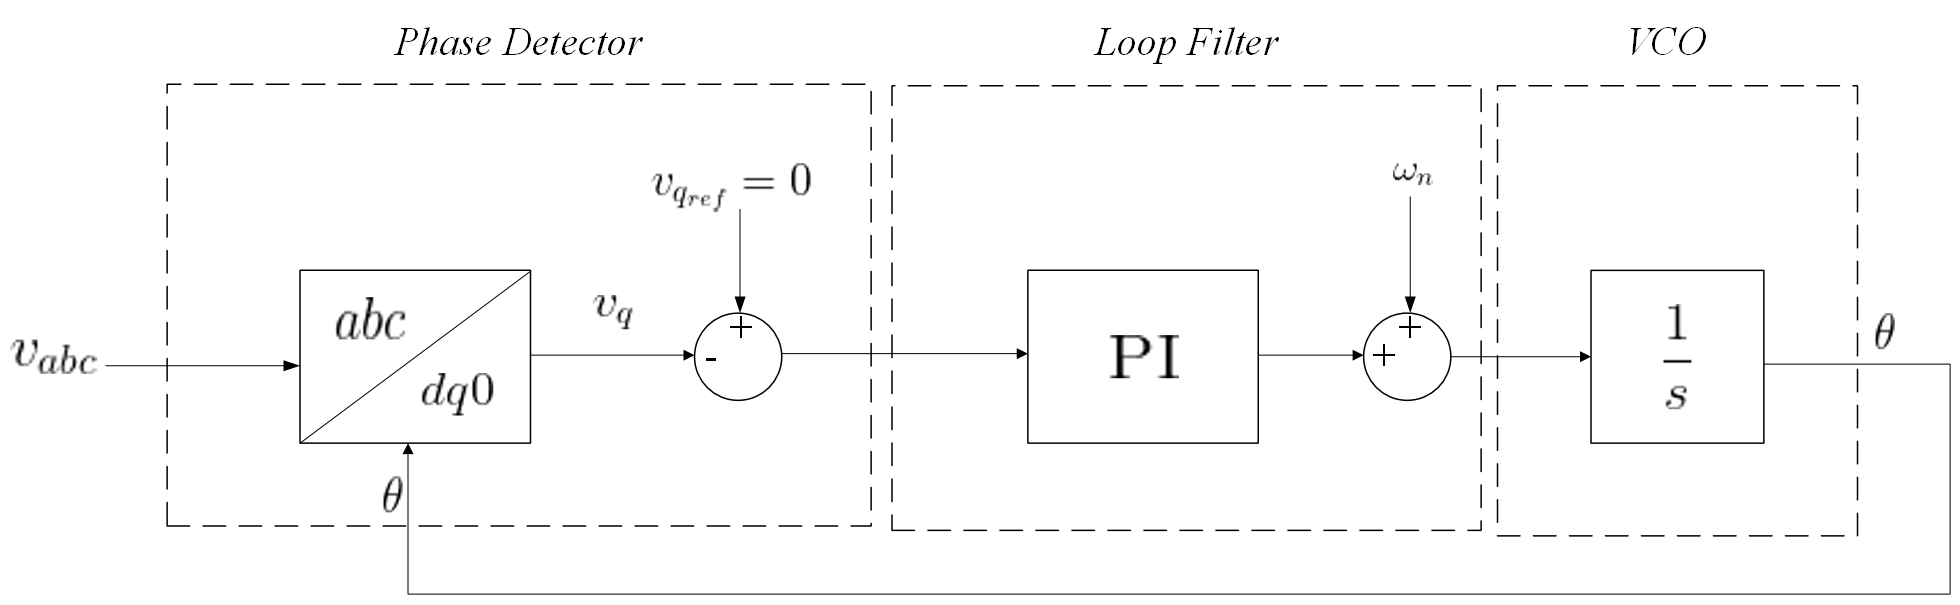
\includegraphics[width=0.95\linewidth]{Images/PLL_Diagram_2024.11.11_OTL.png}
    \caption{A diagram of the PLL}
    \label{fig:PLLDiagram}
\end{figure}

Within a synchronous reference frame phase-locked-loop (SRF-PLL) are three components: the phase-detection mechanism, the loop filter, and the voltage-controlled oscillator (the VCO). \autoref{fig:PLLDiagram} shows the three components. $v_{abc}$ is the three-phase input voltage, $v_q$ is the quadrature voltage in the $dq$ representation of the input voltage, $\omega_n$ is the nominal grid frequency, and $\theta$ is the estimated grid phase. In three-phase SRF-PLLs, the phase detection mechanism accepts a three-phase signal, determines its phase, and compares it to the estimated phase signal.

The loop filter is generally a PI (proportional-integral) controller with control law

\begin{equation}
    \frac{k_p s + k_i}{s}
\end{equation}

Finally, it can proven that the VCO is an integrator \cite{Blaabjerg_Grid_Synchronization}. Literature has shown that the SRF-PLL is a second-order system (i.e., a system with two open-loop poles). Therefore, it can track a constant reference signal with zero steady-state error; however, it cannot track a ramp signal without steady state error \cite{Guerrero_Vasquez_3PLL}. 

\subsection{Synchronization between a Weak Microgrid and a Strong Grid}

Substantial research has been done on synchronization between a "small" grid or power system and a much larger one \cite{Blaabjerg_Grid_Synchronization, Blaabjerg_Microgrids_Control, Guerrero_Hierarchical}.

\subsection{Synchronization between Two Microgrids}

Some work has been done to analyze the interlinking of several microgrids. For example, \cite{Blaabjerg_Interlinking} considers the linking between a single-phase AC microgrid and a DC microgrid. 

The reference \cite{Blaabjerg_Microgrids_Control} discusses synchronization within the “weak” three-phase microgrid as being effected with two types of PLLs: either the SRF-PLL discussed within the previous section or a synchronous reference frame frequency locked loop (SRF-FLL). SRF-PLLs are said to work well when the grid with which to be synchronized has a balanced signal; in contrast, more advanced PLLs are required for signals that are distorted. In contrast, SRF-FLLs are said to be less responsive to phase-angle jumps in the synchronizing signal, making it more desirable in the event of a distorted signal. However, the SRF-FLL’s architecture is more complex than the SRF-PLL’s. 

\section{Research Gaps}

Potential research gaps exist in areas including synchronization quality and consideration of the use of more robust PLLs, and modulation schemes. For example, simulation data for an AC-DC power converter has shown that the SVPWM algorithm can be used in an effective manner to implement bidirectional power transfer \cite{Deng}. Simulation data shows that converters that make use of the SVPWM algorithm have more robust dynamic and steady-state response \cite{Wang}. Finally, with regards to DC-AC power conversion, the SVPWM algorithm makes greater use of available DC voltage in comparison to SPWM, another commonly used modulation scheme \cite{Zhang}.